% all-in-one cheatsheet layout (Michael Franzen, 2013)
\documentclass[a4paper]{article}

% geometry settings
\usepackage[top=2cm, bottom=2.5cm, left=2cm, right=2cm]{geometry}

% font settings
%\usepackage[light,math]{kurier}
\usepackage[T1]{fontenc}
\usepackage[utf8]{inputenc}
\usepackage{marvosym}
\usepackage{amssymb}
\usepackage{amsfonts}
\usepackage{amsmath}
\usepackage{amsthm}

% colors
\usepackage{xcolor}
\definecolor{lightgray}{gray}{0.8}

% formatting
\usepackage{paralist}
\usepackage{multicol}
\usepackage{tabularx}
\usepackage{Tabbing}
\usepackage{booktabs}
\usepackage{fancyhdr}
\usepackage{url}
\usepackage[framemethod=tikz]{mdframed}
\pagestyle{fancy}

% math
\usepackage{array}
\usepackage{eqnarray}
\usepackage{mathtools}

% figures
\usepackage{wrapfig}
\usepackage{subfig}

% figure modules
\usepackage{graphicx}
\usepackage{tikz}
\usetikzlibrary{positioning,calc, shapes}
\usepackage{algorithm2e}
\usepackage{verbatim}	

% TOC & Glossary
\usepackage{sectsty}
\usepackage[nottoc,notlof,notlot]{tocbibind}
\usepackage[titles,subfigure]{tocloft}

% commands
\usepackage{xargs}
\usepackage{ifthen}

% head line
\fancyhf{}
\chead{Graph Theory - Sheet 2 - \today\\J. Batzill (1698622), M. Franzen (1696933), J. Labeit (1656460)}
\renewcommand{\headrulewidth}{0.4pt} %obere Trennlinie

\newcommand{\sheetnumber}{1}

% (problem number)
\surroundwithmdframed[
    hidealllines=true,
    backgroundcolor=gray!10,
    skipbelow=\baselineskip,
    skipabove=\baselineskip
]{mylemma}

\surroundwithmdframed[
	linecolor=white,
	skipbelow=\baselineskip,
	skipabove=\baselineskip
]{mytheorem}




\begin{document}
	
	\newtheorem{mytheorem}{Theorem}[section]
	\newtheorem{mylemma}{Lemma}[mytheorem]	

	\newenvironmentx*{solution}[1]{\section*{Problem #1}\addtocounter{section}{1}\setcounter{mylemma}{0}\setcounter{mytheorem}{0}}{}
	\newenvironmentx*{theorem}[1]{\begin{mytheorem}#1\\\begin{proof}}{\end{proof}\end{mytheorem}}
	\newenvironmentx*{lemma}[1]{\begin{mylemma}#1\\\begin{proof}}{\end{proof}\end{mylemma}}


	\begin{solution}{5}
		\begin{theorem}{Let $G$ be a nonempty graph with minimum degree at least two. Then, there is a connected graph $G'$ having the same degree sequence as $G$.}

			We will show that we are able to inter-connect any two components of $G$ without changing the graph's degree-sequence. We accomplish this by choosing two adjacent vertices in each component and modify the incident edges such that the components are connected. Finally, we will show that our modification does not change any vertex degree, nor does it disconnect any component. Inductively, we are then able to connect any graph $G$ without changing any degree (and therefore without changing the degree sequence).\\

			\begin{center}
				\resizebox {0.25\textwidth}{!}{
					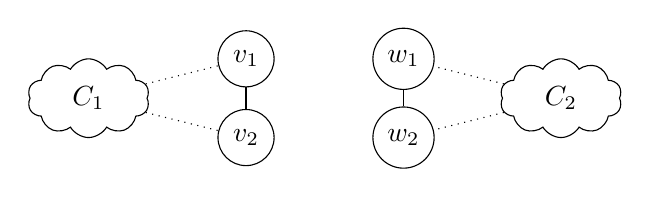
\begin{tikzpicture}
						\node[cloud, cloud puffs=10, cloud puff arc=120, aspect=2, minimum width=1.5cm, minimum height=1cm, draw] (c1)  at (-1,-0.5) {$C_1$};
						\node[circle, draw] (v1) at (1, 0) {$v_1$};
						\node[circle, draw] (v2) at (1, -1) {$v_2$};
						\draw[dotted] (c1) -- (v1);
						\draw[dotted] (c1) -- (v2);
						\draw (v1) -- (v2);
		
						\node[cloud, cloud puffs=10, cloud puff arc=120, aspect=2, minimum width=1.5cm, minimum height=1cm, draw] (c2)  at (5,-0.5) {$C_2$};
						\node[circle, draw] (w1) at (3, 0) {$w_1$};
						\node[circle, draw] (w2) at (3, -1) {$w_2$};
						\draw[dotted] (c2) -- (w1);
						\draw[dotted] (c2) -- (w2);
						\draw (w1) -- (w2);
					\end{tikzpicture}
				} $\Rightarrow$
				\resizebox {0.25\textwidth}{!}{
					\begin{tikzpicture}
						\node[cloud, cloud puffs=10, cloud puff arc=120, aspect=2, minimum width=1.5cm, minimum height=1cm, draw] (c1)  at (-1,-0.5) {$C_1$};
						\node[circle, draw] (v1) at (1, 0) {$v_1$};
						\node[circle, draw] (v2) at (1, -1) {$v_2$};
						\draw[dotted] (c1) -- (v1);
						\draw[dotted] (c1) -- (v2);
						\draw (v1) -- (w1);
		
						\node[cloud, cloud puffs=10, cloud puff arc=120, aspect=2, minimum width=1.5cm, minimum height=1cm, draw] (c2)  at (5,-0.5) {$C_2$};
						\node[circle, draw] (w1) at (3, 0) {$w_1$};
						\node[circle, draw] (w2) at (3, -1) {$w_2$};
						\draw[dotted] (c2) -- (w1);
						\draw[dotted] (c2) -- (w2);
						\draw (w1) -- (w2);
					\end{tikzpicture}
				} $\Rightarrow$
				\resizebox {0.25\textwidth}{!}{
					\begin{tikzpicture}
						\node[cloud, cloud puffs=10, cloud puff arc=120, aspect=2, minimum width=1.5cm, minimum height=1cm, draw] (c1)  at (-1,-0.5) {$C_1$};
						\node[circle, draw] (v1) at (1, 0) {$v_1$};
						\node[circle, draw] (v2) at (1, -1) {$v_2$};
						\draw[dotted] (c1) -- (v1);
						\draw[dotted] (c1) -- (v2);
						\draw (v1) -- (w1);
		
						\node[cloud, cloud puffs=10, cloud puff arc=120, aspect=2, minimum width=1.5cm, minimum height=1cm, draw] (c2)  at (5,-0.5) {$C_2$};
						\node[circle, draw] (w1) at (3, 0) {$w_1$};
						\node[circle, draw] (w2) at (3, -1) {$w_2$};
						\draw[dotted] (c2) -- (w1);
						\draw[dotted] (c2) -- (w2);
						\draw (v2) -- (w2);
					\end{tikzpicture}
				}
			\end{center}

			Let $C_1 = (V_1, E_1)$ and $C_2 = (V_2, E_2)$ be components of $G$. Furthermore, we consider $v_1, v_2 \in V_1$ to be adjacent vertices contained in a cycle of $C_1$ and $w_1, w_2 \in V_2$ to be adjacent vertices contained in a cycle of $C_2$. We always find those vertices since the graph's minimum degree exceeds or is equal to two (Lecture: \emph{Any graph $H$ with $\delta(H) \geq 2$ contains a cycle}).\\

			First, we remove the edges $\{v_1, v_2\} \in E_1$ and $\{w_1, w_2\} \in E_2$. Notably, neither $C_1$ nor $C_2$ have been disconnected since each of these edges is contained in a cycle and hence not crucial for the connectivity of $C_1$ and $C_2$. Now, we add the edges $\{v_1, w_1\}$ as well as $\{v_2, w_2\}$ and thereby connect $C_1$ with $C_2$.\\
			
			We can easily see that no degree has been changed. Each vertex has lost and gained one incident edge. From these considerations, the graph's degree sequence has not been modified. Moreover, we have connected the two components without disconnecting one.

			Inductively, we are able to connect the entire graph and at the same time maintain it's degree sequence. Thus, a connected graph with the same degree sequence exists.

		\end{theorem}
	\end{solution}
	\newpage
	\begin{solution}{6}
		In the following, I will proof that any tree with an even number of vertices has exactly one spanning subgraph in which every vertex has odd degree. 
		I will reduce the problem by recursively removing leaves until only the trivial case of two vertices is left. 
		First, I will proof the following lemma which then later is used to proof the theorem. 
			
		\begin{lemma}{Let $T=(V,E)$ be a tree with $|V|>2$. If there is no vertex $u \in V$ connected to at least two leaves $v_1, v_2 \in V$, there is a leaf $v \in V$ connected to a vertex $u$ with $d(u) = 2$.}
			From the prerequisite that there is no vertex $u \in V$ connected to at least than two leaves, we know that all leaves are connected to different vertices. 
			Let's assume that there is no such vertex $u$, then all vertices $u \in V$ connected to a leaf must not have a degree of two ($d(u) \neq 2$). 
			Because $T$ is connected and $|V|>2$, all $u$ must have an edge and cannot be a leaf itself. Hence, for all such $u$, $d(u) \geq 3$. 
			By removing all leaves from $T$, we get $T'$ a subgraph of $T$. By removing the leaves, only the degree of all $u$ connected to a leaf are reduced by one. 
			Then, for all $u$, $d(u) \geq 2$ in the subgraph $T'$. 
			Additionally, because the degree of all other vertices is not changed and they are no leaves, the degree of all vertices of the resulting graph is greater or equal to two. 
			Thus, using a lemma of the lecture, the resulting graph must have a cycle (Lecture: \emph{Any graph $H$ with $\delta(H) \geq 2$ contains a cycle}). 
			Because $T'$ is a subgraph of $T$, this is a contradiction to $T$ being acyclic. Hence, there has to be a vertex $u$ connected to a leaf with $d(u)=2$. 		
		\end{lemma}
					
		\begin{theorem}{Any tree with an even number of vertices has exactly one spanning subgraph in which every vertex has odd degree.}
			Let $T=(V, E)$ be a tree with an even number of vertices. If $|V|=2$ there is obviously exactly one spanning subgraph. 
			In the following, let $|V|>2$ and let $S$ be the set of edges of a spanning subgraph meeting the conditions stated above. \\
			In the lecture we proved that $T$ has at least one leaf $v$. 
			Because any leaf only $v$ has exactly one edge $(v,u)$, this edge has to be in $S$. 
			Additionally, if the edge $(v,u)$ is in $S$ the condition that the degree of any vertex is odd is met for the leaf $v$. 
			Then, always one of the following cases applies. 
			\begin{itemize}
				\item \textbf{Case 1:} There is one vertex $u \in V$ connected to atleast two leaves $v_1, v_2 \in V$. \\
				We know that the edges $(u,v_1)$ and $(u,v_2)$ have to be in $S$, because $v_1$ and $v_2$ are leaves. 
				If we remove $v_1$ and $v_2$ from T we again receive a tree $T'$ with an even number of vertices. 
				Additionally, if there is exactly one spanning subgraph for $T'$ with only odd degrees then there is also exactly one for $T$ which additionally covers the vertices $v_1$ and $v_2$. 
				Hence, either $|V- \{v_1,v_2\}| \leq 2$ and we know that there is exact one spanning subgraph meeting the conditions, or we can again apply case 1 or case 2. 
				
				\begin{center}
				\resizebox {0.25\textwidth}{!}{
					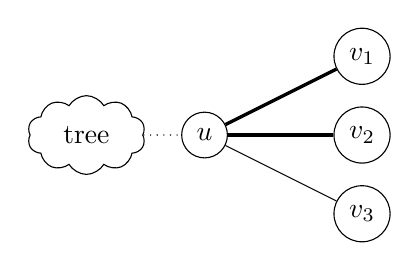
\begin{tikzpicture}
						\node[cloud, cloud puffs=10, cloud puff arc=120, aspect=2, minimum width=1.5cm, minimum height=1cm, draw] (c1)  at (-2.5,-0.5) {tree};
						\node[circle, draw] (u) at (-1, -0.5) {$u$};
						\node[circle, draw] (v1) at (1, 0.5) {$v_1$};
						\node[circle, draw] (v2) at (1, -0.5) {$v_2$};
						\node[circle, draw] (v3) at (1, -1.5) {$v_3$};
						\draw[very thick] (u) -- (v1);
						\draw[very thick] (u) -- (v2);
						\draw (u) -- (v3);
						\draw[dotted] (c1) -- (u);

					\end{tikzpicture}
				} $\Rightarrow$
				\resizebox {0.25\textwidth}{!}{
					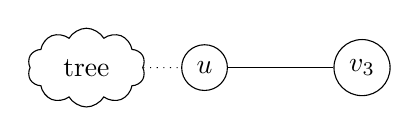
\begin{tikzpicture}
						\node[cloud, cloud puffs=10, cloud puff arc=120, aspect=2, minimum width=1.5cm, minimum height=1cm, draw] (c1)  at (-2.5,-0.5) {tree};
						\node[circle, draw] (u) at (-1, -0.5) {$u$};
						\node[circle, draw] (v3) at (1, -0.5) {$v_3$};
						\draw (u) -- (v3);
						\draw[dotted] (c1) -- (u);
					\end{tikzpicture}
				}
			\end{center}
			
				
				\item \textbf{Case 2:} There is no vertex $u \in V$ connected to atleast two leaves $v_1, v_2 \in V$. \\
				Using the lemma we can find a leaf $v \in V$ with an edge $(v,u) \in E$ with $deg(u)=2$. 
				We know that the edge $(v,u)$ has to be in $S$, because $v$ is a leaf. 
				Additionally, we know that the degree of $u$ in any spanning subgraph meeting the conditions has to be odd, so the second edge $(u,t)$ with $t \in V$ cannot be in $S$. 
				If we remove $u$ and $v$ from T we again receive a tree with an even number of vertices. 
				Hence, either $|V- \{v,u\}| \leq 2$ and we know that there is exact one spanning subgraph meeting the conditions, or we can again apply case 1 or case 2. 
				\begin{center}
				\resizebox {0.25\textwidth}{!}{
					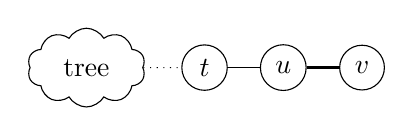
\begin{tikzpicture}
						\node[cloud, cloud puffs=10, cloud puff arc=120, aspect=2, minimum width=1.5cm, minimum height=1cm, draw] (c1)  at (-2.5,-0.5) {tree};
						\node[circle, draw] (t) at (-1, -0.5) {$t$};
						\node[circle, draw] (u) at (0, -0.5) {$u$};
						\node[circle, draw] (v) at (1, -0.5) {$v$};
						\draw[dotted] (c1) -- (t);
						\draw (t) -- (u);			
						\draw[very thick] (u) -- (v);

					\end{tikzpicture}
				} $\Rightarrow$
				\resizebox {0.25\textwidth}{!}{
					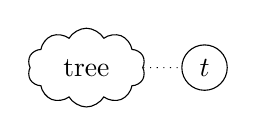
\begin{tikzpicture}
						\node[cloud, cloud puffs=10, cloud puff arc=120, aspect=2, minimum width=1.5cm, minimum height=1cm, draw] (c1)  at (-2.5,-0.5) {tree};
						\node[circle, draw] (t) at (-1, -0.5) {$t$};
						\draw[dotted] (c1) -- (t);
					\end{tikzpicture}
				}
			\end{center}
			\end{itemize}
		All in all, we can always find edges in $T$ which have to be in $S$ and thus we can reduce $T$ uniquely, until there is only the trivial solution. 
		Thus, the theorem is proven by induction. 
		\end{theorem}
	\end{solution} 
	\newpage
	\begin{solution}{7}
		\begin{theorem}{
		For a set $C = \{G_1, ..., G_n\}$ of connected components ($G_i = (V_i, E_i), i = 1..n$) of a graph $G$ let $\pi(C)$ denote the minimum number of walks on $C$ so that every edge of G appears once in exactly one walk and does not appear in other walks.\\
		\begin{align}
			I&=\{i \in \{1,...,n\} |\ E_i \neq \emptyset\}&\\
			\pi(C)&= \sum_{i \in I} \max(\frac{|\{v \in V(G_i)\ |\ d(v) \text{ odd}\}|}{2}, 1)&
		\end{align}}			
			First, for a graph $G$, we build $\pi(G_i)$ for each connected component of $G$ and afterwards summarize these component-bound values. This applies since no walk between each component exists and thus the minimum number of such walks cannot deceed the built sum.

			Let $G_i$ be a connected component in $C$ and $P$ be the set of walks forming such a minimum cover.
			
			\begin{itemize}
				\item \textbf{Case 1: $G_i$ has at least one odd-degree vertex.}\\
					First, we show that each odd-degree vertex in $G_i$ is the endpoint of at least one walk $p \in P$.\\

					We assume $u$ is of odd degree and not an endpoint of any walk $p \in P$.
					Then, $p$ only runs \emph{over} $u$ and thus covers  for each passing of $u$ exactly two of it's incident edges.  In other words, only an even amount of $u$-incident edges can be covered by such a walk $p$.
					Thus, there is one remaining edge incident to $u$ not covered by any walk. This is contradictory, our assumption is false and therefore: \emph{Any odd-degree vertex is the endpoint of at least one walk $p \in P$}.\\
			
			 		Next, we show that no even vertex $v_1 \in V_i$ is an endpoint of a walk $p = (v_1, ..., v_n) \in P$.
					\begin{itemize}
						\item \textbf{Case 1: $p$ is not a cycle.} Considering that $p$ is not a cycle, then the number of non-$p$-covered edges incident to $v_1$ is odd. As shown above, we find a walk $p' \in P$ ($p \neq p'$) starting in $v$. However, then we were able to decrease the amount of walks by fusing $p$ with $p'$. A contradiction to the minimum-size property of $P$. Hence, \emph{there is no even-degree vertex that is an endpoint of a non-cyclic walk in $P$}.
						\item \textbf{Case 2: $p$ is a cycle.} On the other hand, assuming that $p$ is a cycle ($v_1 = v_n$), then - since each vertex passing of $p$ covers exactly two edges - there has to be at least one edge $e = \{w_j, v_p\} \in E_i\ (w \in v_p)$ not covered by $p$ (since $G_i$ has an odd-degree vertex). Since all edges have to be covered by at least one walk in $P$, there must exists a walk $p' = (w_1, ..., w_j,w_{j+1} = v_p, ..., w_m) \in P$ running over $e$. However, we are again able to fuse $p$ with $p'$  by constructing a walk $(w_1, ..., w_j, v_p, ..., v_n = v_1, ..., v_p = w_{j+1}, ..., w_m)$. This is again contradictory to the minimum-size property of $P$. Hence, \emph{there is no even-degree vertex that is an endpoint of a cycle in $P$}.
					\end{itemize}
					By these considerations, \emph{there is no even-degree vertex that is an endpoint of a walk in $P$}.
					
					All in all, each odd-degree vertex is the endpoint of at least one walk in $P$ and thereby is the number of remaining non-covered edges incident to this vertex even. Therefore - as shown above - it cannot be the endpoint of any more walks in $P$.\\

					From these considerations, any odd-degree vertex is exactly one endpoint of exactly one walk in $P$ and furthermore, every endpoint of a walk in $P$ is an odd-degree vertex. \textbf{Thus, for every two odd-degree vertices we have one walk in $P$}.
			
				\item \textbf{Case 2: $G_i$ has no odd vertices.}
					If there is no odd-degree vertex, all edges $G_i$ are covered by \textbf{exactly one walk}, the Euler tour. In summary, we get exactly one walk. In case that $E_i = \emptyset$, there are no walks required.
			\end{itemize}
			All in all, our set of walks consists of one walk for each pair of odd-degree vertices and one walk for every component consisting of only even-degree vertices (which have at least one edge). This equals the expression stated above.
		\end{theorem}
	\end{solution}
	
\end{document}
